
\documentclass[a4paper,10pt]{article}
\usepackage[utf8]{inputenc} %Codificacion utf-8
\usepackage{graphicx}
\usepackage{enumerate}
\usepackage{fancyhdr}
\usepackage{hyperref}
\usepackage{multirow} % Required for multirows
\usepackage[spanish, activeacute]{babel} %Definir idioma español
% \usepackage[margin=3cm]{geometry}
\hypersetup{
    colorlinks=true,
    linkcolor=black,
    filecolor=magenta,
    urlcolor=cyan,
}
\pagestyle{fancy}

\lhead{Análisis clínicos III}
\rfoot{Página \thepage}
\lfoot{Diego Rodríguez Riera}
\cfoot{Bases de Datos}
\newcommand\tab[1][1cm]{\hspace*{#1}}

\title{Análisis clínicos III}
\author{Diego Rodríguez Riera}
\date{22 de Septiemnbre de 2018}

\begin{document}

\maketitle
\pagebreak
\tableofcontents
\pagebreak

\section{Definición del problema.}
\paragraph{}
A lo largo de las clases impartidas el alumnado ha comprendido la importancia de una descripción rigurosa del problema del mundo real con el fin de poder construir un modelo conceptual del mismo que sirva de base para la representación lógica del problema y su tratamiento mediante la tecnología de bases de datos.
\paragraph{}
Por lo tanto, como paso previo al uso de un modelo de datos para la construcción del modelo conceptual, es necesario llevar a cabo el estudio exhaustivo del problema planteado (Gestión de Análisis Clínicos).
\paragraph{}
En este estudio se describirán todos los elementos de información que participan en el problema, su definición, descripción y medida, así como las relaciones existentes entre los elementos de información.
\paragraph{}
Además, se consideraran las restricciones innatas al problema existentes en los elementos de información y las relaciones que existen entre los mismos.
\paragraph{}
Dado que aún no han sido impartidos los conceptos sobre el modelo conceptual Entidad-Interrelación, en esta actividad no se utilizará este modelo para la descripción del problema. Se trata que el alumnado estudie, comprenda y describa el problema, y los elementos de información que deben considerarse y sus características teniendo en cuenta los procesos que deberán considerarse para la gestión de esta información.
\pagebreak

\section{Análisis del problema.}
\paragraph{}
El problema esta planteado en el dominio de los análisis clínicos con metodos actuales, estos se centran en varios factores los cuales varían según la edad, sexo y enfermedades del cliente.
\paragraph{}
Estos factores supondrán en gran parte la complejidad de la base de datos, especificamente el dominio de los datos de la base de datos en los cuales tendrán que estar representadas en estas restricciones.
\section{Factores a tener en cuenta.}
\paragraph{}
Los factores que más influyen en un análisis clínico son los siguientes:
\begin{itemize}
	\item Edad.
	\item Sexo.
	\item Embarazo.
	\item Enfermedades.
	\item Consumo de cafeína, tabaco o alcohol.
	\item Situaciones de estrés o ansiedad.
	\item Ejercicio Físico antes de la realización de la prueba.
\end{itemize}

\section{Mediciones recogidas por los análisis.}
Las medidas que se obtendrán serán las siguientes según el tipo de  análisis:
\subsection{Analisis de sangre.}
Glucosa, Colesterol total, Colesterol HDL, Colesterol LDL, Triglicéridos, Ácido úrico, Transaminasas, GOT/ASAT, GPT/ALT, Proteínas totales, Albúmina, Bilirrubina total, Hematíes (eritrocitos), Hemoglobina, Hematocrito, V.C.M., H.C.M., C.H.C.M., Leucocitos, Neutrófilos, Linfocitos, Monocitos, Eosinófilos, Basófilos, Hierro, Ferritina, Plaquetas, V.S.G., Fibrinógeno \subsection{Analisis de saliva.}
pH, Sodio, Potasio, cloro
\subsection{Analisis de orina.}
Albúmina, Densidad, pH, Glucosa, Proteínas, Cetonas, Urobilinógeno y bilirrubina, Nitrito, Cristales, Células epiteliales, cilindros, Cuerpos cetónicos, Osmolalidad, Glóbulos rojos, Glóbulos blancos, Cetona, Creatinina
\pagebreak

\section{Diagrama de abstracción de análisis.}
\paragraph{}
Para poder implementar todas las restricciones de dominio, tendremos que crear el siguiente árbol de generalización para los analisis:\\
\vspace{0.7cm}\\
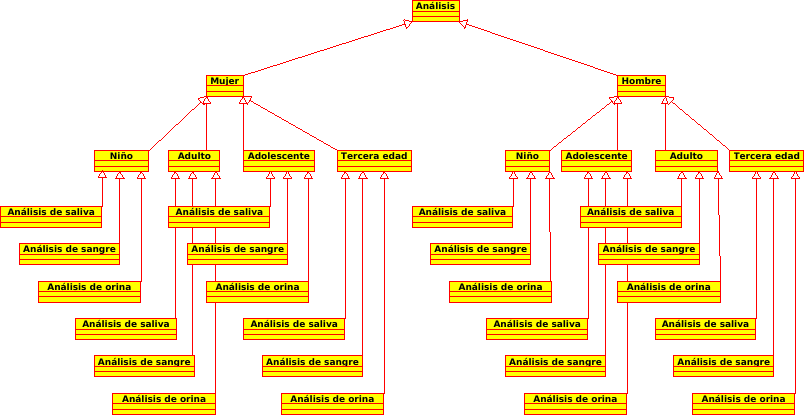
\includegraphics[width=\textwidth]{img/analisis.png}
\paragraph{}
Estas clases, a demás de las mediciones obtenidas por el análisis, tendrán también unos valores máximos y mínimos saludables para cada una de las mediciones evaluadas en los distintos análisis para su posterior contraste de resultados por el médico.
\paragraph{}
En el caso de la mujer, habrá dos máximos y mínimos, uno para el estado no embarazada y otro para el estado embarazada, se aplicaran uno u otro dependiendo de la variable booleana "embarazada".
\paragraph{}
Antes de la impresión, se evaluara si la medición esta entre los parametros máximos y mínimos, si esta no lo esta la medición se marcará en otro color al del texto.
\paragraph{}
Nótese que solo el sexo, edad, y en el caso de la mujer, si esta está embarazada se han tenido en cuneta para los máximos y los mínimos, el resto de factores se almacenaran en la variable "observaciones" en las clases, para su posterior consideración por el personal cualificado.
\pagebreak

\section{Diagrama de abstracción de personas.}
\paragraph{}
Hay tres tipos de personas, el paciente al que se realiza el análisis, el Doctor que receta el análisis el analista que lleva a cabo el análisis en el laboratorio.
\paragraph{}
El diagrama de abstracción seria el siguiente:
\vspace{0.5cm}
\begin{center}
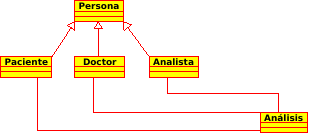
\includegraphics{img/personas.png}
\end{center}
\paragraph{}
Para que un análisis sea realizado este debe de ser mandado por un médico a excepción de casos particulares.
\paragraph{}
Las propiedades que se guardarán de las distintas clases serán las siguientes:
\begin{itemize}
	\item {\bf Paciente}: dni, numero de la seguridad social, sexo, fecha de nacimiento, lugar de nacimiento y una lista de análisis realizados.
	\item {\bf Doctor}: dni, fecha de nacimiento y campo o especialidad.
	\item {\bf Analista}: dni, fecha de nacimiento, campo o especialidad y especialidad como analista.
\end{itemize}
\paragraph{}
Tanto los médicos como los analistas tendrán estar titulados con las titulaciones correspondientes a la tarea desempeñada, y el dni del paciente tendrá que ser válido.
\paragraph{}
cada análisis tiene un id único, este es generado automáticamente y es incremental, además, el análisis guarda de quien es el análisis (paciente), quien lo ha realizado (analista) y quien lo ha encargado (el doctor).
\paragraph{}

\pagebreak

\section{Diagrama de abstracción de máquinas.}
En el laboratorio existen tres tipos de maquinas que pueden escribir o leer de un análisis, estas están representadas en el siguiente diagrama:
\vspace{0.5cm}\\
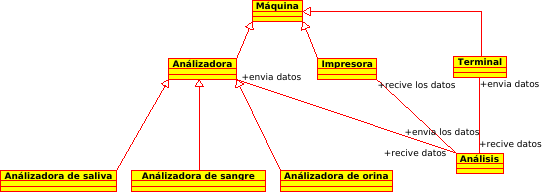
\includegraphics[width=\textwidth]{img/maquinas.png}
\paragraph{}
Como se puede observar, de la clase maquina, derivan tres subclases:
\begin{itemize}
	\item {\bf Análizadora} Maquina encargada de obtener automáticamente los análisis de las muestras del paciente, hay tres tipos, una por cada tipo de análisis:
	\begin{itemize}
		\item {\it Análizadora de sangre}.
		\item {\it Análizadora de saliva}.
		\item {\it Análizadora de orina}.
	\end{itemize}
	Estas maquinas pueden obtener ciertos resultados por ellas mismas sin intervención humana mas allá del posicionamiento de las muestras.
	\item {\bf Impresora}: Encargada de imprimir todo documento que se le mande.
	\item {\bf Terminal}: Debido a que no todas las mediciones podrán hacerse automáticamente por las máquinas, algunas muestras tendrán que ser analizadas por los analistas, estos entonces podrán introducir los resultados a travez de una terminal en el laboratorio.
\end{itemize}
\paragraph{}
Una vez completado el análisis, se mandara un documento generado a partir de los datos del análisis al servidor de impresión para su posterior recogida por el doctor que la encargo.\\
\pagebreak
\section{Vista general.}
\paragraph{}
Gran parte del diagrama de análisis ha sido omitido.\\
\vspace{0.7cm}\\
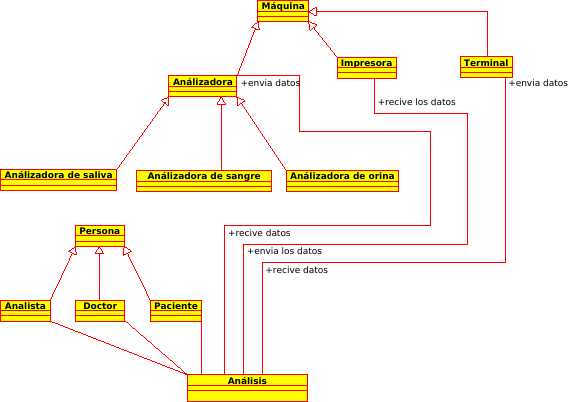
\includegraphics[width=\textwidth]{img/all.png}




%%%%%%%%%%%%%%%%%%%%%%%%%%%%%%%%%%%%%%%%%%%%%%%%%%%%%%%%%%%%%%%%%%%%%%%%%%%%%%%%
%%%%%%%%%%%%%%%%%%%%%%%%%%%%%%%%%%%%%%%%%%%%%%%%%%%%%%%%%%%%%%%%%%%%%%%%%%%%%%%%
%                           commented out things
%%%%%%%%%%%%%%%%%%%%%%%%%%%%%%%%%%%%%%%%%%%%%%%%%%%%%%%%%%%%%%%%%%%%%%%%%%%%%%%%
%%%%%%%%%%%%%%%%%%%%%%%%%%%%%%%%%%%%%%%%%%%%%%%%%%%%%%%%%%%%%%%%%%%%%%%%%%%%%%%%




% \section{Tabla de valores aceptables}
% \subsection{Análisis de sangre}
% \begin{center}
% 	\begin{tabular}{|c|c|c|c|c|c|c|c|c|c|} \hline
%
% 		% header
%
% 		\multirow{2}{*}{medida} & \multicolumn{4}{|c|}{Hombre} & \multicolumn{4}{|c|}{Mujer} & \multirow{2}{*}{unidades} \\ \cline{2-9}
% 		& 0-10 & 10-20 & 20-50 & 50+ & 0-10 & 10-20 & 20-50 & 50+ & \\ \hline
%
% 		% data
%
% %Glucosa,
%
% Glucosa & 100-180 & \multicolumn{3}{|c|}{90-130} & 100-180 &  \multicolumn{3}{|c|}{90-130} & mg/dL \\ \hline
% Colesterol total & \multicolumn{2}{c|}{$<$170} & \multicolumn{2}{c|}{125-200} &\multicolumn{2}{c|}{$<$170} & \multicolumn{2}{c|}{125-200} & mg/dL\\ \hline
% Colesterol HDL  &\multicolumn{4}{c|}{$<$100} &\multicolumn{4}{c|}{$<$100} & mg/dL\\ \hline
% Triglicéridos &  &  &  &  &  &  & & & \\ \hline
% Ácido úrico &  &  &  &  &  &  & & & \\ \hline
% Transaminasas &  &  &  &  &  &  & & & \\ \hline
% GOT/ASAT &  &  &  &  &  &  & & & \\ \hline
% GPT/ALT &  &  &  &  &  &  & & & \\ \hline
% Proteínas totales &  &  &  &  &  &  & & & \\ \hline
% Albúmina &  &  &  &  &  &  & & & \\ \hline
% Bilirrubina total &  &  &  &  &  &  & & & \\ \hline
% Hematíes (eritrocitos) &  &  &  &  &  &  & & & \\ \hline
% Hemoglobina &  &  &  &  &  &  & & & \\ \hline
% Hematocrito &  &  &  &  &  &  & & & \\ \hline
% V.C.M. &  &  &  &  &  &  & & & \\ \hline
% H.C.M. &  &  &  &  &  &  & & & \\ \hline
% C.H.C.M. &  &  &  &  &  &  & & & \\ \hline
% Leucocitos &  &  &  &  &  &  & & & \\ \hline
% Neutrófilos &  &  &  &  &  &  & & & \\ \hline
% Linfocitos &  &  &  &  &  &  & & & \\ \hline
% Monocitos &  &  &  &  &  &  & & & \\ \hline
% Eosinófilos &  &  &  &  &  &  & & & \\ \hline
% Basófilos &  &  &  &  &  &  & & & \\ \hline
% Hierro &  &  &  &  &  &  & & & \\ \hline
% Ferritina &  &  &  &  &  &  & & & \\ \hline
% Plaquetas &  &  &  &  &  &  & & & \\ \hline
% V.S.G. &  &  &  &  &  &  & & & \\ \hline
% Fibrinógeno &  &  &  &  &  &  & & & \\ \hline
%
%
% 	\end{tabular}
% \end{center}


% \raggedleft Document written in \LaTeX{}
\end{document}
